%Chapter5
\chapter{Requirement}
\label{Chapter5}
In the project there was the need for a deep analysis of all the tied requirements. The result of this analysis was essential to identify the subsequent problems.\\
We will describe all of them, distinguishing between functional and nonfunctional requirements.
\section{Functional}
\subsection{Connection management with the acquisition device}
Fundamental feature to be included inside the mobile application is the capability to directly connect the smartphone device to the acquisition device ZEcg. Since this last one was designed to transmit the signals through a bluetooth channel, we have to implement and manage a bluetooth socket connection inside the application in order to receive the data.
\subsection{Acquisition, storing and management of ECG records}
For a matter of medical feature as it is a fact that there are many “standards” on saving an ECG signal, the application has to be able to manage different formats. Even though this application is designed to be used mostly for acquisition from the ZEcg device, it is also able to open and read other standard format such as the MIT-BIH, one of the most common standard in the literature of ECG. The code software behind is designed in a such  way that the integration of other format is made extremely easy to add just by implementing few interfaces and classes.

\subsection{Different ECG formats support}
For a matter of medical feature as it is a fact that there are many “standards” on saving an ECG signal, the application has to be able to manage different formats. Even though this application is designed to be used mostly for acquisition from the ZEcg device, it is also able to open and read other standard format such as the MIT-BIH, one of the most common standard in the literature of ECG. The code software behind is designed in a such  way that the integration of other format is made extremely easy to add just by implementing few interfaces and classes.

\subsection{Dynamic display scaling}
The mobile device market is huge and there are a very large number of devices with completely different hardware and screens. As first classification we can distinguish mobile devices into smartphones and tablets. The most obvious difference is based on the screen size and the pixel density. Building a mobile application means also to deal with these number of different devices. To achieve the same experience and look and feel the application should be able to scale its view according to the device screen and the pixel density. A typical ECG signal is plot on a paper with squares of well defined size in millimeters. The mobile application has to respect such a standard independently on the screens capabilities and pixel density, so it should be able to properly scale the view and the plotting based on the hardware provided by the device.

\subsection{ECG record analysis integration on mobile platform}
To complete the set of features for the application we plan to integrate the algorithms of ECG signal processing. To have a mobile device able not only to acquire and visualize in real time the ECG but also to analyze it at runtime, can be of vital importance, especially if the user has little knowledge about reading and interpreting an ECG graph. The integrated algorithms for arrhythmia analysis are based on a Neural Network trained to recognized the nature of the signals for the given record with high accuracy. The algorithms come from a previous thesis work\cite{ref3} which belongs to Ulisse Pizzagalli, student at Politecnico of Milan.
\subsection{Analysis results displaying}
After analysis there are results that need to be shown to the user in the most friendly and understandable way. The most important results from an ECG analysis are called Istogram, Tacogram and the ST+/ST- . They are respectively graphs showing the number of heart rates of a certain value, the average heart rate at each heart beat and the difference between the area ST+ and ST-, the area above the segment ST and the one below. This last graph is useful for ischemia detection.\cite{ref4}
\begin{figure}[ht!]
	\centering
	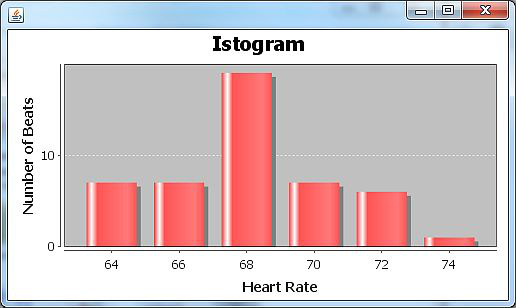
\includegraphics[width=90mm]{figures/ch5/1.png}
	\caption{Istogram from the desktop application resulted from an analysis on a MIT/BIH record.}
	\label{fig5.1}
\end{figure}
\begin{figure}[ht!]
	\centering
	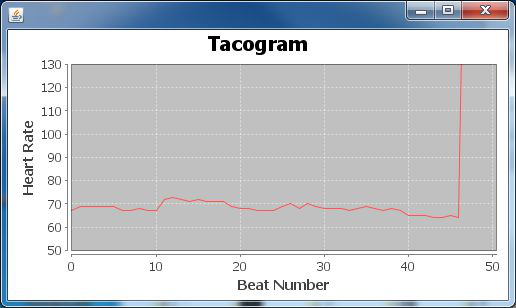
\includegraphics[width=90mm]{figures/ch5/2.png}
	\caption{Tacogram from the desktop application resulted from an analysis on a MIT/BIH record.}
	\label{fig5.2}
\end{figure}
\begin{figure}[ht!]
	\centering
	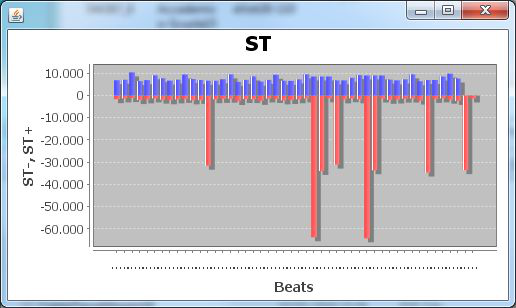
\includegraphics[width=90mm]{figures/ch5/3.png}
	\caption{ST+/ST- graph from the desktop application resulted from an analysis on a MIT/BIH record.}
	\label{fig5.3}
\end{figure}

\subsection{Highly parameterizable}
We believe in dynamic software, that is why we planned from the beginning on making this application dynamic. Even if the application is  build on top of the ZEcg standard, we plan to make the software responsive also to other standards. To achieve this, we planned to abstract all the acquisition device independent features and functionalities. In order to support as much as possible any variants of the original acquisition device, we plan to setup customizable parameters, the only related to the hardware implementation. With a little of changes the application will be able to interface with other devices as well for acquisition.

\section{Nonfunctional}
\subsection{Reduced memory usage}
This requirement is fundamental for any project related to mobile application development. In fact, if a desktop pc in general doesn’t have any problem related to memory usage (even if it is a good practice not to waste memory), on mobile devices this over-usage can bring the application to crash and get killed by the OS. The memory available is higher on new devices with respect to older ones,  but it is still small so it is always a good practice to use it carefully.
\subsection{Minimum performance rate and scalability on performance}
Nowadays the new high level mobile devices has quad-core or even octa-core cpu processors. Any application should take advantage of a such configuration, but on the other hand mobile application developers should always consider the fact that the market is still full of older and low-end devices. In order to cover at least most of the market devices their application have to run fine (with a minimum acceptable performance rate) starting from the low-end devices and, at the same time, taking advantage of last devices capabilities. \\
We believe modern applications should seriously take this aspect in consideration, because it will make their application scalable also from a performance point of view.
\subsection{ Wide platform compatibility and accessibility}
Developing a mobile application implies building a software that has to be executed on many different platforms. The smartphone and tablet market is huge with many different devices mounting different hardwares and running of the three major mobile OS (iOS, Android and Windows Phone). In the next chapters we will deal with this issue.   
\subsection{Documentation}
This thesis includes also a more technical documentation about the development phase and the choices we starting from the planning phase to the development phase. The software is fully documented and with annotations and comments to increase code readability and future development on top of it. The technical documentation is included in the next chapters where we are going to discuss and motivate the implementation and the results.